\documentclass{article}

\usepackage{amsmath, amsthm, amssymb}
\usepackage{graphicx}

\title{Notes for MATH 3210: Foundation of Analysis I}
\author{Jing Guo}
\date{\today}

\begin{document}

    \maketitle
    \tableofcontents
    
    \section{Ring and Field}
    
    Notations:
    
    \begin{itemize}
        \item $\mathbb{N}$: The set of natural numbers;
        \item $\mathbb{Z}$: The set of integers (ring, not field, has no inverse);
        \item $\mathbb{Q}$: The set of rational numbers;
        \item $\mathbb{R}$: The set of real numbers (ring and field).
    \end{itemize}
    
    \subsection{Ring}
    
    The set $A$ has two binary operations, addition and multiplication.
    
    For any $a, b \in A$,
    
    \begin{align*}
        A \ast A &\to A \\
        a, b &\to a + b
    \end{align*}
    
    \subsubsection{Addition Axiom}

    \begin{enumerate}
        \item $a + b = b + a$ (commutative)
        \item $(a + b) + c = a + (b + c)$ (associative)
        \item There is an element $0$ such that $a + 0 = a$ (additive identity)
        \item There exists $-a$ (additive inverse) such that $a + (-a) = 0$
    \end{enumerate}

    \subsubsection{Multiplication Axiom}
    
    \begin{enumerate}
        \item $a \cdot b = b \cdot a$
        \item $(a \cdot b) \cdot c = a \cdot (b \cdot c)$
        \item There is an element $1$ such that $a \cdot 1 = a$ and $0 \neq 1$
        \item $a \cdot (b + c) = a \cdot b + a \cdot c$ (distributive)
    \end{enumerate}

    \subsection{Field}
    
    $A$ is a field if $A$ is a \textit{ring} for any $a \in A$ and $a \neq 0$, there exists $a^{-1}$ (inverse of $a$) such that $a \cdot a^{-1} = 1$.
    
    $A$ has no zero divisors if $x \neq 0, y \neq 0 \rightarrow x \cdot y \neq 0$
    
    \textbf{Example}: $x, y \in A$, $x \neq 0$, $y \neq 0$, $xy = 0$
    
    \begin{displaymath}
    \begin{bmatrix}
        1 & 0 \\
        0 & 0
    \end{bmatrix}
    \cdot
    \begin{bmatrix}
        0 & 0 \\
        0 & 1
    \end{bmatrix}
    =
    \begin{bmatrix}
        0 & 0 \\
        0 & 0
    \end{bmatrix}
    \end{displaymath}
    
    \subsection{Construction of Integers}
    
    We need to construct $\mathbb{Z}$ from $\mathbb{N}$ with \textbf{localization}.
    
    \begin{displaymath}
        \mathbb{N} = \{ 0, 1, 2, 3, \ldots \}
    \end{displaymath}
    
    Set of equivalence class: $\mathbb{N} \times \mathbb{N} / \sim$
    
    Equivalence relation: $(a, b) \sim (a', b')$ if $a + b' = b + a'$, since $a - b = a' - b'$
    
    \begin{gather*}
        (a, b) \sim (a', b') \sim (a'', b'') \\
        a' + b'' = b' + a'' \\
        \boldsymbol{(a + b'') + b'} = (a + b') + b''
        = b + a' + b'' = b + b' + a'' = \boldsymbol{(a'' + b) + b'} \\
        \therefore a + b'' = a'' + b \\
        \therefore (a, b) \sim (a'', b'')
    \end{gather*}
    
    We then should define addition:
    
    \begin{equation} \label{eq:add1}
        [(a, b)] + [(a', b')] = [(a + a', b + b')]
    \end{equation}
    
    \begin{equation} \label{eq:add2}
        [(a_{1}, b_{1})] + [(a', b')] = [(a_{1} + a', b_{1} + b')]
    \end{equation}
    
    Equation \ref{eq:add1} and equation \ref{eq:add2} are equal since independent of choice of equivalence classes:
    
    \begin{gather*}
        a + a' + b_{1} + b' = a_{1} + a' + b + b' \\
        a + b_{1} = a_{1} + b
    \end{gather*}
    
    Additive identity: $0 = [(0, 0)]$
    
    For example: $[(a, b)] + [(b, a)] = [(a + b, a + b)] = [(0, 0)] = 0$
    
    We then need to define multiplication:
    
    \begin{displaymath}
        [(a, b)] \cdot [(a', b')] = [(aa' + bb', ab' + a'b)]
    \end{displaymath}
    
    \begin{align*}
        &(a - b)(a' - b') \\
     = \quad &aa' - ab' - a'b + bb' \\
     = \quad &(aa' + bb') - (ab' + a'b)
    \end{align*}
    
    Multiplicative identity: $1 = [(1, 0)]$
    
    For example: $[(a, b)] \cdot [(1, 0)] = [(a, b)]$
    
    $\therefore \mathbb{N} \times \mathbb{N} / \sim$ is a ring, that is, $\mathbb{Z}$.
    
    \begin{align*}
        \mathbb{N} &\longrightarrow \mathbb{Z} \\
        m &\longrightarrow [(m, 0)] \\
        -m &\longrightarrow [(0, m)] = -[(m, 0)]
    \end{align*}
    
    For example:
    
    \begin{align*}
        [(a, b)] &= [(a, 0)] + [(0, b)] \\
                   &= [(a, 0)] - [(b, 0)]
    \end{align*}
    
    \subsection{Construction of Fractions (Rational Numbers)}
    
    We need to show that $K$ is a field (with addition and multiplication). Assume $A$ is a commutative ring with no zero divisors, and $A^{\ast} = A - \{ 0 \}$.
    
    $A \times A^{\ast} = \{ (a, b) \mid a, b \in A, b \neq 0 \}$
    
    Set of equivalence classes: $K = (A \times A^{\ast}) / \sim$ (elements of $K$ are fractions)
    
    We first need to define addition:
    
    \begin{align*}
        (a, b) &\sim (a', b') \\
        \frac{a}{b} &= \frac{a'}{b'} \\
        ab' &= a'b
    \end{align*}
    
    $[(a, b)]$: The equivalence class of $(a, b)$
    
    \begin{align*}
        [(a, b)] + [(a', b')] &= [(ab' + a'b, bb')] = \frac{ab' + a'b}{bb'} \\
        [(0, 1)] &= 0 \in K \quad \text{(additive identity)} \\
    \end{align*}
    
    The following is to prove that it is independent of the choice of equivalence class:
    
    \begin{align*}
        [(a_{1}, b_{1})] + [(a', b')] &= [(a_{1}b' + a'b_{1}, b_{1}b')] \\
        \therefore (ab' + a'b) \cdot b_{1}b' &= (a_{1}b' + a'b_{1}) \cdot bb' \\
        \therefore left &= right
    \end{align*}
    
    We then need to define multiplication:
    
    \begin{align*}
        [(a, b)] [(a', b')] &= [(aa', bb')] = \frac{aa'}{bb'} \\
        [(1, 1)] &= 1 \in K \quad \text{(multiplicative identity)}
    \end{align*}
    
    \textbf{Examples}:
    
    \begin{align*}
        [(x, y)] + [(0, 1)] = [(x, y)] \\
        [(x, y)] \cdot [(1, 1)] = [(x, y)] \\
        [(x, y)] \neq [(0, 1)]
    \end{align*}
    
    So we need to show that $K$ is a field:
    
    \begin{align*}
        [(x, y)] \cdot [(y, x)] &= [(xy, xy)] = [(1, 1)] \quad \text{(Non-zeros have inverse)} \\
        \because &ab' = a'b \\
                       &(a, b) \sim (a', b') \\
        \therefore &[(xy, xy)] = [(1, 1)]
    \end{align*}
    
    \textbf{Therefore} $K$ is a field of fractions of $A$.
    
    We need to show the following map is injective:
    
    If $A = \mathbb{Z}$ and $K = \mathbb{Q}$:
    
    \begin{align*}
        A &\longrightarrow K \quad \text{{(injective)}} \\
        x &\longrightarrow [(x, 1)] \\
        x + y &\longrightarrow [(x + y, 1)] = [(x, 1)] + [(y, 1)] \\
        x \cdot y &\longrightarrow [(xy, 1)] = [(x, 1)] \cdot [(y, 1)] \\
        \text{Comm. ring without } 0 &\longrightarrow \text{Field containing the ring}
    \end{align*}

    Assume $[(a, 1) = [(b, 1)]]$ where $a, b \in A$:
    
    \begin{align*}
        &a \cdot 1 = b \cdot 1 \Rightarrow a = b \\
        &\therefore \text{The map is injective.}
    \end{align*}
    
    $P(x) = a_{0}x^{n} + a_{1}x^{n - 1} + a_{2}x^{n - 2} + \cdots + a_{n}, a \in R$
    
    Ring of polynomials: $P(x) \times Q(x) \Rightarrow R(x)$ (with no zero divisors)
    
    \subsection{Ordered Set}
    
    \subsubsection{Partial Order}
    
    $(S, \leq)$ is a (partially) ordered set (poset), $\forall x, y, z \in S$:
    
    \begin{enumerate}
        \item $x \leq$ x
        \item $x \leq y, y \leq x \Rightarrow x = y$
        \item $x \leq y, y \leq z \Rightarrow x \leq z$
    \end{enumerate}

    \subsubsection{Total Order}

    Total/Linear order: Either $x \leq y$ or $y \leq x$.
    
    Ordered field is a field $K$ with $\leq$ total order.
    
    \textbf{Definition}:
    
    \begin{enumerate}
        \item If $x \leq y$ then $x + z \leq y + z$ and
        \item if $x \geq 0, y \geq 0$ then $x \times y \geq 0$
    \end{enumerate}

    \textbf{First example}:
    
    \begin{gather*}
        \mathbb{Q} = \{ (a, b) \}, (a, b) = \frac{a}{b} \\
        \text{Since} \quad a \geq 0, b > 0
    \end{gather*}
    
    $\therefore \mathbb{Q}$ is an ordered set.
    
    \textbf{Second example}:
    
    \begin{align*}
        x \geq 0 &\Leftrightarrow -x \leq 0 \\
        x \geq 0 &\Rightarrow x^{2} \geq 0 \\
        x \leq 0 &\Rightarrow (-x)^{2} = x^{2} \geq 0
    \end{align*}
    
    \begin{align*}
        1^{2} = 1 > 0 \\
        2 > 1 \\
        3 > 2 \\
        \vdots \\
        n > n - 1
    \end{align*}
    
    \subsubsection{Least-upper-bound Property}
    
    $\mathbb{Q}$: Ordered field of rational numbers (with gaps)
    
    Least-upper-bound property: $K$ has least-upper-bound property if any bounded subset $E \subset K$ has least upper bound.
    
    $K$ is a field with order relation $\leq$, $E \subset K$ and $E$ is \textit{bounded above} if $\exists \alpha \in K$ such that $p \leq \alpha, p \in E$.
    
    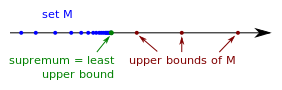
\includegraphics{supremum}
    
    $\beta$ is the \textit{least-upper-bound} of $E$ if
    
    \begin{enumerate}
        \item $\beta$ is an upper bound,
        \item for any other upper bound $\alpha$, we have $\beta \leq \alpha$.
    \end{enumerate}

    We call $\beta = \sup E$.
    
    We then need to prove that $\mathbb{Q}$ does not have least-upper-bound property, that is, there are gaps in $\mathbb{Q}$.
    
    \begin{proof}
            \begin{align*}
                E = \{ q \in \mathbb{Q} : q^{2} \leq 2 \} \quad &\Rightarrow \quad  \text{no } \sup E \\
                q \in E \Leftrightarrow - q \in E \quad &\text{and} \quad q \geq 0 \\
            \end{align*}
            
            Let $p \in \mathbb{Q}$ such that $p \geq 0, p^{2} > 2$.
            $\therefore p^{2} > 2 \geq q^{2} \Rightarrow p^{2} \geq q^{2}$
    \end{proof}

    \section{Basic Topology}

        Metric (distance function) of $x_{0}$ and $x$: $d(x_{0}, x) = \lvert x - x_{0} \rvert$

    \subsection{Metric Space $M$}

        \begin{displaymath}
        d \colon M \times M \to \mathbb{R}
        \end{displaymath}

        \begin{enumerate}
            \item $d(x_{0}, x_{1}) \geq 0$ where $x_{0}, x_{1} \in M$
            \item $d(x_{0}, x_{1}) = 0 \iff x_{0} = x_{1}$
            \item $d(x_{0}, x_{1}) = d(x_{1}, x_{0})$ (irrespective of order)
            \item $d(x, z) \leq d(x, y) + d(y, z)$ (triangular inequity)
        \end{enumerate}

        Euclidean metric on $\mathbb{R}^{2}$:
        $d(x, y) = \sqrt{(x_{1} - y_{1})^{2} + (x_{2} - y_{2})^{2}}$

        Discrete metric: $d(x, y) = \left\{\begin{matrix}
        1 &\mbox{if}\ x \neq y \\
        0 &\mbox{if}\ x = y 
        \end{matrix}\right.$

        Open ball of radius $\epsilon$:
        $B_{\epsilon}(x_{0}) = B(x_{0}, \epsilon) = \{ y \in M \mid d(x_{0}, y) < \epsilon \}$

    \subsection{Open Sets}

        \subsubsection{Metric Spaces $X$}

        $U \subset X$ is open if for any $x \in U$ there exists $\epsilon > 0$ such that $B(x, \epsilon) \subset U$.

        Open interval is open set; closed interval is not open set.

        \subsubsection{Topological Spaces $(X, U)$}

        Let $U$ be a family of all sets, $X$ be a set. $U$ is a \textbf{topology} on $X$ if

        \begin{enumerate}
            \item $\emptyset$ (Empty set) is always open; $X$ is open. $\Leftrightarrow$ $\emptyset$ and $X$ itself belong to $U$.
            \item $F$ is a collection of open sets, then $\bigcup_{U \in F} U$ is open. $\Leftrightarrow$ Any union of members of $U$ still belongs to $U$. (Union)
            \item $F$ is a \textit{finite} collection of open sets, then $\bigcap_{U \in F} U$ is open. $\Leftrightarrow$ The intersection of any finite number of members of $U$ belongs to $U$. (Intersection)
        \end{enumerate}

        Finite case: $x \in \bigcap_{U \in F} U$, $x \in U$, hence $B(x, \epsilon_{U}) \subset U$

        \begin{gather*}
            \delta = \min \epsilon_{U} > 0 \quad where \quad U \in F \\
            B(x, \delta) \subset B(x, \epsilon_{U}) \subset U \\
            \therefore B(x, \delta) \subset \bigcap_{U \in F} U
        \end{gather*}

        Infinite case: For example, the intersection of all intervals of $( -\frac{1}{n}, \frac{1}{n})$, where $n$ is a positive number, is the set $\{ 0 \}$ which is not open in the real line.

    \subsection{Compact Sets}

        In metric space $X$, compact sets are \underline{closed}.

        Compact $\Leftrightarrow$ closed and bounded (only for Euclidean metric, $\mathbb{R}^{n}$)

\end{document}